\documentclass{article}

%Vamos importar um pacote
\usepackage[brazil]{babel}
\usepackage{graphicx}
\usepackage[round,authoryear,sort]{natbib}

%Corpo
% Onde a gente escreve o texto
%%%%%%%%%%%%%%%%%%%%%%%%%%%%%
\begin{document}

\title{Análise da variação de temperatura dos últimos cinco anos}
\author{Eric Frota de Sousa}

%Cria o título
\maketitle

\begin{abstract}
Meu resumo!
\end{abstract}

\section{Introdução}
Isso vai ser a inha introdução.
Outra frase.

Esse já é outro parágrafo.

Trabalhos anteriores bem legais fizeram coisas parecidas
\citep{Hansen2010}.
Isso foi analisado primeiro por \citet{Hansen2010}

\section{Metodologia}
\label{sec:metodos}

Aqui vou descrever tudo o que eu fiz.
Ajustamos uma reta aos cinco últimos anos dos dados
de emperatura média mensal para cada país.
Assim calculamos a taza de variação de temperatura recente.



\begin{equation}
y = \int\Omega x dx
\end{equation}

A equação da reta é

\begin{equation}
T(t) = a t + b,
\label{eq:reta}
\end{equation}

\noindent
onde $T$ é a temperatura , $t$ é o tempo, $a$ é o coeficiente angular
e $b$ é o coeficiente linear.

Utilizamos a equação \ref{eq:reta} em um código Python para fazer o ajuste da
reta com o método dos mínimos quadrados.
Isso está descrito na seção \ref{sec:metodos}.

%Meu primeiro artigo em LaTeX

\section{Resultados}

Analisamos os dados de 225 países. São muitos para listar aqui.

\begin{figure}
%\begin{figure}[!htb]
	%\centering
	%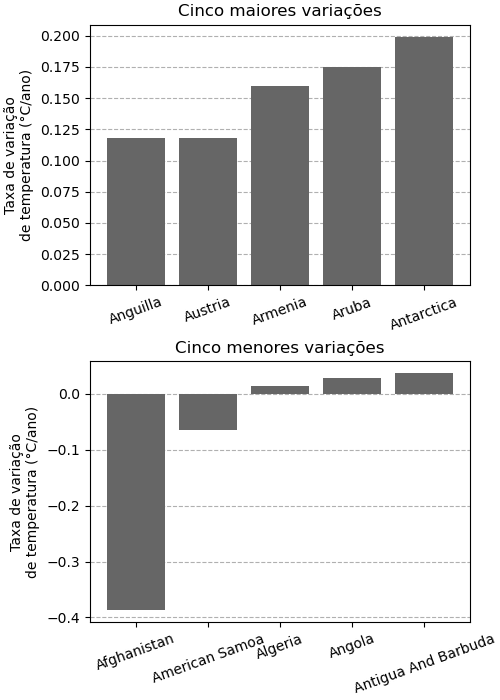
\includegraphics[width=0.5\columnwidth]{../figuras/variacao_temperatura.png}
	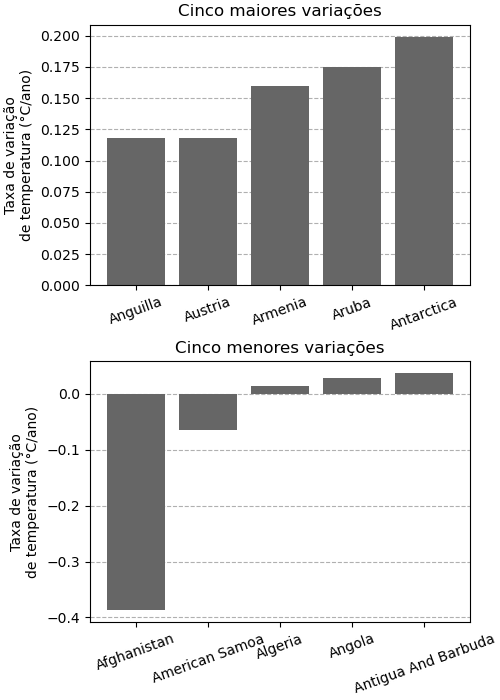
\includegraphics{../figuras/variacao_temperatura.png}
	\caption{
	Variação de temperatura média mensal dos últimos cinco anos.
	a) Países com as cinco maiores variações de temperatura.
	b) Países com as cinco menores variações de temperatrua.	
	}
	\label{fig:variacao}
\end{figure}

Os resultados da análise de variação de termperatura estão na figura \ref{fig:variacao}

%Referências
\bibliographystyle{apalike}
\bibliography{referencias.bib}

\end{document}